\documentclass[a4paper]{article}

\usepackage[sc]{mathpazo}
\usepackage{parskip}
\usepackage{microtype}
\usepackage[utf8]{inputenc}
\usepackage{inconsolata}
\usepackage{appendix}
\usepackage{color}
\usepackage[usenames,svgnames]{xcolor}
\usepackage{listings}
\usepackage{fancyvrb}
\usepackage{titlesec}
\usepackage{graphicx}
\usepackage{titling}
\usepackage{nag}
\usepackage[margin=1.3in]{geometry}

\newcommand{\sectionbreak}{\clearpage}

\makeatletter
\def\PY@reset{\let\PY@it=\relax \let\PY@bf=\relax%
    \let\PY@ul=\relax \let\PY@tc=\relax%
    \let\PY@bc=\relax \let\PY@ff=\relax}
\def\PY@tok#1{\csname PY@tok@#1\endcsname}
\def\PY@toks#1+{\ifx\relax#1\empty\else%
    \PY@tok{#1}\expandafter\PY@toks\fi}
\def\PY@do#1{\PY@bc{\PY@tc{\PY@ul{%
    \PY@it{\PY@bf{\PY@ff{#1}}}}}}}
\def\PY#1#2{\PY@reset\PY@toks#1+\relax+\PY@do{#2}}

\expandafter\def\csname PY@tok@gu\endcsname{\def\PY@tc##1{\textcolor[rgb]{0.67,0.67,0.67}{##1}}}
\expandafter\def\csname PY@tok@gt\endcsname{\def\PY@tc##1{\textcolor[rgb]{0.67,0.00,0.00}{##1}}}
\expandafter\def\csname PY@tok@gs\endcsname{\let\PY@bf=\textbf}
\expandafter\def\csname PY@tok@gr\endcsname{\def\PY@tc##1{\textcolor[rgb]{0.67,0.00,0.00}{##1}}}
\expandafter\def\csname PY@tok@cm\endcsname{\let\PY@it=\textit\def\PY@tc##1{\textcolor[rgb]{0.60,0.60,0.53}{##1}}}
\expandafter\def\csname PY@tok@vg\endcsname{\def\PY@tc##1{\textcolor[rgb]{0.00,0.50,0.50}{##1}}}
\expandafter\def\csname PY@tok@m\endcsname{\def\PY@tc##1{\textcolor[rgb]{0.00,0.60,0.60}{##1}}}
\expandafter\def\csname PY@tok@mh\endcsname{\def\PY@tc##1{\textcolor[rgb]{0.00,0.60,0.60}{##1}}}
\expandafter\def\csname PY@tok@go\endcsname{\def\PY@tc##1{\textcolor[rgb]{0.53,0.53,0.53}{##1}}}
\expandafter\def\csname PY@tok@ge\endcsname{\let\PY@it=\textit}
\expandafter\def\csname PY@tok@gd\endcsname{\def\PY@tc##1{\textcolor[rgb]{0.00,0.00,0.00}{##1}}\def\PY@bc##1{\setlength{\fboxsep}{0pt}\colorbox[rgb]{1.00,0.87,0.87}{\strut ##1}}}
\expandafter\def\csname PY@tok@il\endcsname{\def\PY@tc##1{\textcolor[rgb]{0.00,0.60,0.60}{##1}}}
\expandafter\def\csname PY@tok@cs\endcsname{\let\PY@bf=\textbf\let\PY@it=\textit\def\PY@tc##1{\textcolor[rgb]{0.60,0.60,0.60}{##1}}}
\expandafter\def\csname PY@tok@cp\endcsname{\let\PY@bf=\textbf\def\PY@tc##1{\textcolor[rgb]{0.60,0.60,0.60}{##1}}}
\expandafter\def\csname PY@tok@gi\endcsname{\def\PY@tc##1{\textcolor[rgb]{0.00,0.00,0.00}{##1}}\def\PY@bc##1{\setlength{\fboxsep}{0pt}\colorbox[rgb]{0.87,1.00,0.87}{\strut ##1}}}
\expandafter\def\csname PY@tok@gh\endcsname{\def\PY@tc##1{\textcolor[rgb]{0.60,0.60,0.60}{##1}}}
\expandafter\def\csname PY@tok@ni\endcsname{\def\PY@tc##1{\textcolor[rgb]{0.50,0.00,0.50}{##1}}}
\expandafter\def\csname PY@tok@nn\endcsname{\def\PY@tc##1{\textcolor[rgb]{0.33,0.33,0.33}{##1}}}
\expandafter\def\csname PY@tok@no\endcsname{\def\PY@tc##1{\textcolor[rgb]{0.00,0.50,0.50}{##1}}}
\expandafter\def\csname PY@tok@na\endcsname{\def\PY@tc##1{\textcolor[rgb]{0.00,0.50,0.50}{##1}}}
\expandafter\def\csname PY@tok@nb\endcsname{\def\PY@tc##1{\textcolor[rgb]{0.60,0.60,0.60}{##1}}}
\expandafter\def\csname PY@tok@nc\endcsname{\let\PY@bf=\textbf\def\PY@tc##1{\textcolor[rgb]{0.27,0.33,0.53}{##1}}}
\expandafter\def\csname PY@tok@ne\endcsname{\let\PY@bf=\textbf\def\PY@tc##1{\textcolor[rgb]{0.60,0.00,0.00}{##1}}}
\expandafter\def\csname PY@tok@nf\endcsname{\let\PY@bf=\textbf\def\PY@tc##1{\textcolor[rgb]{0.60,0.00,0.00}{##1}}}
\expandafter\def\csname PY@tok@si\endcsname{\def\PY@tc##1{\textcolor[rgb]{0.73,0.53,0.27}{##1}}}
\expandafter\def\csname PY@tok@s2\endcsname{\def\PY@tc##1{\textcolor[rgb]{0.73,0.53,0.27}{##1}}}
\expandafter\def\csname PY@tok@vi\endcsname{\def\PY@tc##1{\textcolor[rgb]{0.00,0.50,0.50}{##1}}}
\expandafter\def\csname PY@tok@nt\endcsname{\def\PY@tc##1{\textcolor[rgb]{0.00,0.00,0.50}{##1}}}
\expandafter\def\csname PY@tok@nv\endcsname{\def\PY@tc##1{\textcolor[rgb]{0.00,0.50,0.50}{##1}}}
\expandafter\def\csname PY@tok@s1\endcsname{\def\PY@tc##1{\textcolor[rgb]{0.73,0.53,0.27}{##1}}}
\expandafter\def\csname PY@tok@vc\endcsname{\def\PY@tc##1{\textcolor[rgb]{0.00,0.50,0.50}{##1}}}
\expandafter\def\csname PY@tok@gp\endcsname{\def\PY@tc##1{\textcolor[rgb]{0.33,0.33,0.33}{##1}}}
\expandafter\def\csname PY@tok@sh\endcsname{\def\PY@tc##1{\textcolor[rgb]{0.73,0.53,0.27}{##1}}}
\expandafter\def\csname PY@tok@ow\endcsname{\let\PY@bf=\textbf}
\expandafter\def\csname PY@tok@sx\endcsname{\def\PY@tc##1{\textcolor[rgb]{0.73,0.53,0.27}{##1}}}
\expandafter\def\csname PY@tok@bp\endcsname{\def\PY@tc##1{\textcolor[rgb]{0.60,0.60,0.60}{##1}}}
\expandafter\def\csname PY@tok@c1\endcsname{\let\PY@it=\textit\def\PY@tc##1{\textcolor[rgb]{0.60,0.60,0.53}{##1}}}
\expandafter\def\csname PY@tok@kc\endcsname{\let\PY@bf=\textbf}
\expandafter\def\csname PY@tok@c\endcsname{\let\PY@it=\textit\def\PY@tc##1{\textcolor[rgb]{0.60,0.60,0.53}{##1}}}
\expandafter\def\csname PY@tok@mf\endcsname{\def\PY@tc##1{\textcolor[rgb]{0.00,0.60,0.60}{##1}}}
\expandafter\def\csname PY@tok@err\endcsname{\def\PY@tc##1{\textcolor[rgb]{0.65,0.09,0.09}{##1}}\def\PY@bc##1{\setlength{\fboxsep}{0pt}\colorbox[rgb]{0.89,0.82,0.82}{\strut ##1}}}
\expandafter\def\csname PY@tok@mb\endcsname{\def\PY@tc##1{\textcolor[rgb]{0.00,0.60,0.60}{##1}}}
\expandafter\def\csname PY@tok@ss\endcsname{\def\PY@tc##1{\textcolor[rgb]{0.73,0.53,0.27}{##1}}}
\expandafter\def\csname PY@tok@sr\endcsname{\def\PY@tc##1{\textcolor[rgb]{0.50,0.50,0.00}{##1}}}
\expandafter\def\csname PY@tok@mo\endcsname{\def\PY@tc##1{\textcolor[rgb]{0.00,0.60,0.60}{##1}}}
\expandafter\def\csname PY@tok@kd\endcsname{\let\PY@bf=\textbf}
\expandafter\def\csname PY@tok@mi\endcsname{\def\PY@tc##1{\textcolor[rgb]{0.00,0.60,0.60}{##1}}}
\expandafter\def\csname PY@tok@kn\endcsname{\let\PY@bf=\textbf}
\expandafter\def\csname PY@tok@o\endcsname{\let\PY@bf=\textbf}
\expandafter\def\csname PY@tok@kr\endcsname{\let\PY@bf=\textbf}
\expandafter\def\csname PY@tok@s\endcsname{\def\PY@tc##1{\textcolor[rgb]{0.73,0.53,0.27}{##1}}}
\expandafter\def\csname PY@tok@kp\endcsname{\let\PY@bf=\textbf}
\expandafter\def\csname PY@tok@w\endcsname{\def\PY@tc##1{\textcolor[rgb]{0.73,0.73,0.73}{##1}}}
\expandafter\def\csname PY@tok@kt\endcsname{\let\PY@bf=\textbf\def\PY@tc##1{\textcolor[rgb]{0.27,0.33,0.53}{##1}}}
\expandafter\def\csname PY@tok@sc\endcsname{\def\PY@tc##1{\textcolor[rgb]{0.73,0.53,0.27}{##1}}}
\expandafter\def\csname PY@tok@sb\endcsname{\def\PY@tc##1{\textcolor[rgb]{0.73,0.53,0.27}{##1}}}
\expandafter\def\csname PY@tok@k\endcsname{\let\PY@bf=\textbf}
\expandafter\def\csname PY@tok@se\endcsname{\def\PY@tc##1{\textcolor[rgb]{0.73,0.53,0.27}{##1}}}
\expandafter\def\csname PY@tok@sd\endcsname{\def\PY@tc##1{\textcolor[rgb]{0.73,0.53,0.27}{##1}}}

\def\PYZbs{\char`\\}
\def\PYZus{\char`\_}
\def\PYZob{\char`\{}
\def\PYZcb{\char`\}}
\def\PYZca{\char`\^}
\def\PYZam{\char`\&}
\def\PYZlt{\char`\<}
\def\PYZgt{\char`\>}
\def\PYZsh{\char`\#}
\def\PYZpc{\char`\%}
\def\PYZdl{\char`\$}
\def\PYZhy{\char`\-}
\def\PYZsq{\char`\'}
\def\PYZdq{\char`\"}
\def\PYZti{\char`\~}
% for compatibility with earlier versions
\def\PYZat{@}
\def\PYZlb{[}
\def\PYZrb{]}
\makeatother



\lstset{
	basicstyle=\ttfamily,
	keepspaces=true,
	numbers=none,
	showspaces=false,
	showstringspaces=false,
	showtabs=false,
	tabsize=4
}

\begin{document}

\title{Babble}
\author{
Wander Nauta (s1380893)\\
Derk Snijders (s1299212)
}
\date{\today}

\begin{titlepage}
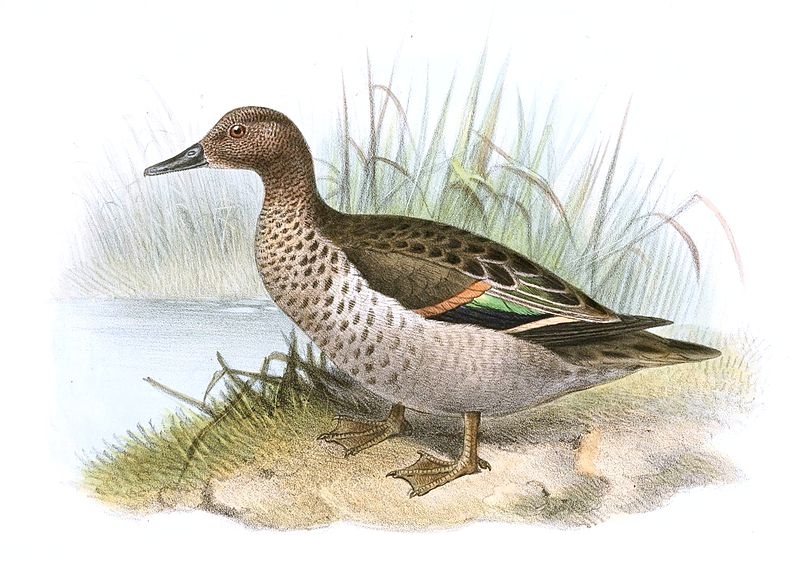
\includegraphics[width=\textwidth]{cover}
\vfill

{\Huge \thetitle}

\theauthor
\end{titlepage}

\tableofcontents

\section{Language summary}
Babble is a compiled, duck-typed, object-oriented programming language for the Java Virtual machine.
It has syntax and semantics inspired by the Smalltalk programming language, but the compile-once-run-anywhere development cycle from Java.
It has no primitives, no operators, no statements like \texttt{if} or \texttt{while}, and no type annotations.
Instead, most everything in Babble is done using message sends.

In Babble, as in Smalltalk, everything is an object, and objects can be interacted with by sending them messages.
If the receiving object understands the message, it acts upon it, sending messages to other objects if required, and finally sending a reply back to the source of the message.
(The process of sending messages would be described as `calling methods' in other languages, while sending a reply would be called `returning a value'.
We use the terms interchangeably.)

Babble is duck typed.
It is a (run-time) error if a receiving object does not understand a message.

Like Smalltalk, Babble has the concept of blocks: pieces of code that can be passed as values.
Blocks can take arguments, and will also do lambda closure.

Babble uses call-by-reference and maintains a scope for variables, this is further augmented using the lambda closure of blocks.

\section{Problems and solutions}
Summary of problems you encountered and how you solved them (max. two
pages).
\subsection{ASM?}
\subsection{Global methods}
\subsection{Passing method arguments}
\subsection{Lambda closure}
\subsection{Multiple files}

Since Babble does not have a lot of special keywords or statements, a large part of what is considered standard functionality is written in Prelude.bla, Babble code, instead. This file was to be included into every other Babble program. Our first solution was to simply concatenate Prelude.bla with the user's program but this caused confusion with locating errors (line numbers where off). A new solution was to generate separate IR trees, and merge them together. Using the TreeMerger class, Babble can read any number of files and combine them into a single IR tree. An added benefit of this is that Babble supports spreading out defining a single class over multiple files. See \ref{merge} for a detailed description of the merging process.

\subsection{While statement}

Babble, like Smalltalk, was designed from the beginning not to have \texttt{if} and \texttt{while} structures in the language, but rather to have these constructs implemented in the language itself.
Once we got blocks working, implementing \texttt{if} was trivial, and indeed the implementations of \texttt{ifTrue:} and \texttt{ifFalse:} on the True and False classes are quite short.

Implementing \texttt{whileTrue}, our version of the while statement, was more involved. The following will result in an infinite loop, which surprised us for a while:

\begin{quote}
\begin{lstlisting}
| i |.
i := 0.

[ i < 20 ] whileTrue: [
	i := i + 1.
].
\end{lstlisting}
\end{quote}

In Babble, most built-in classes are immutable, while references are always mutable. Also, blocks (closures) get their own set of mutable references. Assignments (\texttt{:=}) inside a block will point the variable to a new object, but only inside that block's scope, not outside. This meant that the \texttt{i} variable inside the second block was pointed to ever-increasing numbers, but the \texttt{i} variable inside the first block never changed.

The above is not an issue when working with mutable values, like arrays, which work as expected. Still, because this behaviour could be confusing to people who are not used to programming in Babble (and there are many of those, us included), we recommend using recursion over using \texttt{whileTrue} construct.

\section{Detailed language description}
%A systematic description of the features of your language, for each
%feature specifying
%– Syntax, including one or more examples;
%– Usage: how should the feature be used? Are there any typing or other restrictions?
%– Semantics: what does the feature do? How will it be executed?
%– Code generation: what kind of target code is generated for the feature?
%You may make use of your ANTLR grammar ar as a basis for this description, but note that %not every
%rule necessarily corresponds to a language feature

\subsection{Classes}
A Babble program is a collection of Babble classes.

\subsubsection{Defining classes}
A class is defined by a name, an ID, a possible superclass and then opening brackets. Inside these brackets class fields can optionally be declared using a declaration syntax. Following field declaration are the methods the class has that provide functionality.

Example:
\begin{quote}
\begin{lstlisting}
Duck extends:Animal [
	| age hungry |.
	
	birthday [].
	
	eat: food [].
	
	+: with [].
].
\end{lstlisting}
\end{quote}

Unlike in Java, multiple classes can be defined in a single file, and a single class can be defined in multiple files (see section \ref{merge}). When compiling, each Babble class gets its own metaclass class (see section \ref{metaclass}) and a Java .class file. Declarations are added as fields to the Java class, methods as Java methods.

\subsubsection{Using classes}
\label{metaclass}
After defining a Babble class, new objects of this class can be created. This is done by calling \texttt{new} on the metaclass object belonging to that class. This will then instantiate a new object of the desired class.

Besides the \texttt{new} method, a metaclass object also has \texttt{name methods} and \texttt{respondsTo} methods. \texttt{name} Returns the name of the class ("Duck"), \texttt{methods} returns an array of strings containing the selectors of the methods that the class has. \texttt{respondsTo} Can be used to check if a class has a method.

All Babble classes have a special unary method \texttt{class}. This method returns a metaclass object representing the class. As an alternative, the name of a class can be used to directly refer to a metaclass object of it (\texttt{Duck} as opposed to \texttt{duckInstance class}).


\subsection{Defining methods}

Classes on themselves are quite empty, their functionality is defined inside methods defined in the class. The general syntax is a method name optionally followed by parameters and then a block containing a list of expressions to be executed in order.
There are three different kind of methods, each having slight variations on the general syntax.

Babble methods are translated into Java methods belonging to their corresponding class.


\subsubsection{Unary methods}

A unary method is a method without arguments, an example on how such a method would be defined can be given using the Duck example:

\begin{quote}
\begin{lstlisting}
birthday [
	age := age + 1.
].
\end{lstlisting}
\end{quote}
This method tells the Duck to increment it's age field by 1.

\subsubsection{Keyword methods}
A keyword method is a method with 1 or more arguments, an example on how such a method would be defined can be given using the Duck example:

\begin{quote}
\begin{lstlisting}
eat: food [
	food consume.
	hungry := false.
].
\end{lstlisting}
\end{quote}
This method would tell the food it is consumed and then set the Duck's hungry status to false.

The syntactical difference between unary and keyword methods is in the parameters that the method definition expects. After the name, parameters can be defined using a colon. The name given to the parameter can then be used inside the method body to refer to the value that would be passed as an argument. Following is an example of a multiple-parameter keyword method:

\begin{quote}
\begin{lstlisting}
eat: soup and: potatoes finishWith: dessert [].
\end{lstlisting}
\end{quote}

\subsubsection{Infix methods}

Infix methods probably have the syntax most deviating from the general syntax. Infix method are defined using an operator instead of a identifier as name and always have 1 parameter. An example using the Duck class would be the following:

\begin{quote}
\begin{lstlisting}
+: with [
	(with class name == "Duck") ifTrue: [ Duck new. ].
].
\end{lstlisting}
\end{quote}
This method would return a new Duck when the original Duck is with another Duck.

\subsection{Declaring variables}
Variables in Babble can be declared either as class fields or as local variables in a method. In any case, variables do not have a single type and this is thus not specified. An example would be as follows:
\begin{quote}
\begin{lstlisting}
| variable1 variable2 |.
\end{lstlisting}
\end{quote}

Both classes and methods can optionally declare variables (Although a variable has to be declared before it can be used!). For classes this has to be done before any method definition. In methods, variable declaration can be intertwined with expressions, as long as a variable is declared before usage. Multiple variable declarations of the same name are not allowed.

Babble has 4 special variables, \texttt{true, false, this} and \texttt{nil}. True and false always create a new object of class True or False, this refers to the current object. Nil is a reference to a Nil object, Babble's equivalent of null, indicating the lack of value.
%TODO explain how these are globally available (in software desc).

While the syntax in classes and methods is the same for declaring variables, there is a difference in compiling. Variables declared in classes are added as fields to the JVM class, variables declared in methods are added as local variables to the JVM method.

\

\subsection{Sending messages}

The only way to have a Babble program do anything useful is by sending messages to objects, these messages can be seen as calling a method. Sending a message always returns a value, this is the value of the last expression that was executed in that method. Empty methods return a Nil object.

When running a Babble program, an unary message is send to the main method inside the Babble class that is to be executed, starting the Babble program.

Since Babble is duck typed, there is no compile-time checking whether or not a message send to an object is appropriate. At runtime the message is send to an object. If the object has a method to handle the message everything goes well, in the other case an error occurs if the object does not have a method defined to handle the message sent.

There are again three different kind of messages, each with their own syntax and corresponding to the three method kinds.

\subsubsection{Unary messages}

Unary messages are similar to unary operators from other languages, or zero-argument methods in Java.
The following is an example on how to send a unary message:

\begin{quote}
\begin{lstlisting}
true not.
\end{lstlisting}
\end{quote}

The syntax is straightforward, a 'not' message is to the receiver, a True object.
The receiver will reply with a False object. In other words, this is a unary negation.

\subsubsection{Keyword messages}

Keyword messages are relatively uncommon: they mostly appear in Smalltalk-inspired languages, like Objective-C.
Keyword messages have one or more keywords, one per argument.
These keywords are used to determine which method to call.
For example, the following is a single keyword message:

\begin{quote}
\begin{lstlisting}
array at: 2 put: 10.
\end{lstlisting}
\end{quote}

This sends the message \texttt{at:put:} to the variable \texttt{array}, passing the 2 and 10 as arguments. This would place the number 10 at the third position inside the array.


%TODO method argument passing.

\subsubsection{Infix messages}

Infix messages have selectors that consist entirely of symbols (like `+', `=', or `!'). For example:

\begin{quote}
\begin{lstlisting}
10 > 20.
\end{lstlisting}
\end{quote}

Like other messages, infix messages have exactly one receiver, in this case the integer 10.
Infix messages also have exactly one argument, the integer 20 here.
Because 10 is not larger than 20, the result will be false.

\subsection{Expressions}
%TODO add stuff here.

\subsection{Precedence}

Unary messages have the highest precedence, followed by infix messages, followed by keyword messages. Expressions are evaluated `from left to right'. Precedence can be forced using parenthesis, this can be necessary when having to send a message before applying the result:
\begin{quote}
\begin{lstlisting}
this class name == (that class name)
\end{lstlisting}
\end{quote}
If you leave out the parenthesis, the first class name would be compared to 'that' and the class name of the result of that expression (true or false) would be the value of the entire expression.

There are no special exceptions for `arithmetic' operators: all infix messages share the same precedence.
For example, \texttt{5 + 10 * 2} evaluates to 30, not 25.
To calculate $5 + 10 \times 2$ one would write \texttt{5 + (10 * 2)}.

The precedence rules from arithmetic make sense when doing arithmetic, but since Babble allows classes to provide their own infix methods, the symbols from arithmetic can be used in any context.
For example, `+' is used for string concatenation but also for Duck mating in the Duck example.
The asterisk could  be used as a string repeat method.
In that context, Babble will evaluate an expression like \texttt{"Hello" + "World" * 2} as "HelloWorldHelloWorld": in other words, left to right.

\subsection{Standard classes}

Babble comes with a few built-in classes. Most of these are based on their counterparts in Java.

%TODO Text explaining how these classes are created in Babble (ie: mix of Java classes and Prelude stuff). And how a Babble method call ends in a Java method call (ie: _eqeq_).

%TODO common methods? asString?

\subsubsection{Integers}

Babble supports integers as the only type of number, they can be arbitrary large. Integers are created using a no-decimal number representation in the code. Negative integers can be written down using the conventional representation using a minus sign as a first character. Some examples:
\texttt{1}, \texttt{8589934592} and \texttt{-3}.

As all the objects in Babble are classes, so are integers. An integer has standard methods for the following operators: \texttt{+, -, *, /, \%, ==, >, >=, !=, <=} with these having the expected effect. Additional methods \texttt{min:, max:, abs, negate, signum} are also available as standard methods, each also having the expected effect.

\subsection{Booleans}
In Babble booleans can be created using \texttt{true} or  \texttt{false}, this creates a new object of class True or False respectively. Standard methods for booleans are
\texttt{astString, asint, asBool, not, hashCode, ifTrue:, ifFalse:, ifTrue: ifFalse:, ==, !=, and:, or:, assert}. Most of these are pretty self-explanatory, but there are some which deserve attention. \texttt{ifTrue:} And \texttt{ifFalse:} are the Babble equivalent of an if statement. Depending on which boolean (true or false) the block that is passed as argument gets executed or not. \texttt{ifTrue: ifFalse:} Is Babble's equivalent of an if else statement, acting similar. \texttt{assert} Asserts that the boolean on which this is called is true, offering a convenient way to do integration tests in Babble.


\subsubsection{Strings}

Babble has string literals. String literals are enclosed in double quotes, i.e. \texttt{"Hello, world!"}. Strings have the following standard methods available:

\texttt{upper, lower, starsWith, endsWith:, contains, replace: with:, +, ==, !=}.

\subsubsection{Symbols}

Symbols are written using a hash sign followed by a name, for example: \texttt{\#foo}. Symbols do not need to be declared and are neither integer or string, but there fully own type. Standard methods available for symbols:
\texttt{asInt, asString, ==}. AsInt exposes the internally used index from the symbol, asString returns the full name of the symbol (including the hash sign) as a string.

\subsubsection{Arrays}

Babble offers support for arrays. Arrays can contain any number of objects and grow or shrink automatically when needed and can even contain elements of multiple types. The syntax for array literals is \texttt{1, 2, 3}, \texttt{\#one, "bob", Duck new} or curly brackets with any other type of objects.

Standard methods for arrays are:
\texttt{at:, at: put:, size, isEmpty, notEmpty, add:, addAll:,}
\texttt{first, last,includes:, reverse, asString}. Most of these are self explanatory, \texttt{at:} gets an element at the given index. \texttt{at: put:} Puts a value at a given index, overwriting the previous object at that index. \texttt{add:} Adds an object to the end of the array.


\subsubsection{Blocks}

Blocks can be seen as a group of several expression ordered into one object. Blocks are a class just as other classes and can thus be passed as arguments in the same way that could be done with for example integers.

%TODO Empty Blocks return nothing, creating stack underflow.
Blocks are defined using brackets, containing expressions. An example of this would be:
\texttt{[man setName: "bob". woman setName: "Alice".]}, setting the name of 2 people. (assuming 'man' and 'woman' are valid variables in the scope in which the block is defined.)

%TODO FIX WHILE.
Blocks have 2 standard methods, namely \texttt{value} and \texttt{whileTrue:}. \texttt{value} Executes the expressions contained in the block, and in doing so returns the value of the last expression in the block. \texttt{whileTrue:} Accepts another block and keeps executing that until the block to which \texttt{whileTrue:} was sent returns false.

%TODO Maybe this should be in software description.
Since blocks are classes themselves, a trick is needed to be able to use variables from higher scope, which is in this case other classes. The trick applied is to copy all the variables from the scope in which the block is declared and place them as class fields inside the Block. The resulting effect of this is that Blocks are not able to directly assign new values to variables from higher scope, they can only adapt the variables.

%TODO Block value tricks explained.


\subsection{Tips and tricks}

\subsubsection{Using symbols as enumerations}

\subsubsection{Using blocks as values}

\subsubsection{Using values as blocks}

\subsubsection{Introspection and metaclasses}

Babble offers some amount of introspection into objects: objects can be queried for their class by sending them the \texttt{class} message.
The resulting metaclass instance can then be asked for information about the original class using the \texttt{name} and \texttt{methods} messages.
It can also tell you whether or not the original object will \texttt{respondTo} a certain message.

\label{merge}
\subsubsection{Adding methods to existing classes}

The Babble compiler will merge class definitions with the same name together.
This means that you can extend a class from multiple places in your program.

\subsubsection{Adding methods to metaclasses}

\section{Description of the software}
%Summary of the JAVA classes you implemented; for instance, for symbol
%table management, type checking, code generation, error handling, etc. In your description, rely
%on the concepts and terminology you learned during the course, such as synthesised and inherited
%attributes, tree listeners and visitors

The program itself is a compiler that translates Babble source code into JVM bytecode.
While the compiler does check whether variable names are defined, it can't (and won't try to) do any compile-time type checking.

\subsection{Compiler}

The Babble compiler is split into a front end, a few (relatively small) intermediate passes, and a (relatively large) bytecode generation back end.

\subsubsection{Front end: parser}

Babble's parser is based on ANTLR.
The ANTLR grammar has been included on page \pageref{grammar}.
The resulting parse tree is converted into a tree-based intermediate representation using the visitor on page \pageref{visitor}.

\subsubsection{Intermediate passes}

When the program is parsed, it goes through a few intermediate passes, most of which either annotate the tree representation of the program in some way, or check its semantics.

\textbf{TreeMerger} merges multiple IR trees together into a single IR tree, this is used to add Prelude.bla to the .bla file to compile (or multiple .bla files). This merging however does also happen within a single file, for example when a class definition is spread out over the file.

\textbf{Graphvizitor} generates a visual representation of the merged tree, in the form of .dot files for each Babble class. This file can then be used by dot compiler Graphviz to generate an image.

\textbf{GlobalsGenerator} adds global variables to the tree, such as \texttt{true}, \texttt{false} and \texttt{nil}.

\textbf{MetaclassGenerator} adds metaclasses for each Babble class in the tree.
%TODO more explanation?

\textbf{ScopeChecker} checks if the scope in the generated tree is correct and links Nodes to their Scopes using a ScopeStack. This includes checking if a variable is declared before usage and if there are no duplicate declarations.

\textbf{ScopeStack} keeps track of multiple Scopes (in which variables can be declared), their precedence and thus the correct linking of variables to their declaration.

\subsubsection{Back end: bytecode generator}

The Babble compiler generates Java Virtual Machine bytecode using the ASM bytecode manipulation library from Objectweb.
% ...

\subsection{Runtime environment}

\subsubsection{invokeDynamic}

\section{Test plan and results}
Discussion of the correctness test, using the criteria described in §B.5. You
should provide a set of test programs demonstrating the correct functioning of your compiler. The test
set should contain, next to programs testing the various language featurs, also programs containing
syntactic, semantic or run-time errors.
All tests should be provided as part of the zip-file. One test program should be included as an appendix
in the report (see below).


The Babble compiler itself is tested using unit tests, written in Java, while the runtime system is tested using integration tests, written in Babble.
Both can be executed using Maven by running \texttt{mvn verify}.
Maven can also generate a graphical (HTML) report of the test results using \texttt{mvn site}.
% ...

%TODO tests are divided into the following files/categories...

\section{Conclusions}

\clearpage

\begin{appendices}

\label{grammar}
\section{ANTLR grammar}

\begin{Verbatim}[commandchars=\\\{\}]
\PY{k}{grammar}\PY{+w}{ }\PY{n+nc}{Babble}\PY{p}{;}

\PY{n+nl}{program}\PY{+w}{ }\PY{p}{:}\PY{+w}{ }\PY{n+nv}{clazz}\PY{o}{*}\PY{+w}{ }\PY{p}{;}

\PY{n+nl}{clazz}\PY{+w}{ }\PY{p}{:}\PY{+w}{ }\PY{n+nv}{classname}\PY{o}{=}\PY{n+no}{ID}\PY{+w}{ }\PY{o}{(}\PY{n+no}{EXTENDS}\PY{+w}{ }\PY{l+s}{\PYZsq{}:\PYZsq{}}\PY{+w}{ }\PY{n+nv}{superclass}\PY{o}{=}\PY{n+no}{ID}\PY{o}{)}\PY{o}{?}\PY{+w}{ }\PY{l+s}{\PYZsq{}[\PYZsq{}}\PY{+w}{ }\PY{o}{(}\PY{n+nv}{decls}\PY{+w}{ }\PY{l+s}{\PYZsq{}.\PYZsq{}}\PY{o}{)}\PY{o}{?}\PY{+w}{ }\PY{n+nv}{mthd}\PY{o}{*}\PY{+w}{ }\PY{l+s}{\PYZsq{}].\PYZsq{}}\PY{+w}{ }\PY{p}{;}

\PY{n+nl}{mthd}\PY{+w}{ }\PY{p}{:}\PY{+w}{ }\PY{o}{(}\PY{n+no}{ID}\PY{+w}{ }\PY{l+s}{\PYZsq{}:\PYZsq{}}\PY{+w}{ }\PY{n+nv}{decl}\PY{o}{)}\PY{o}{+}\PY{+w}{ }\PY{l+s}{\PYZsq{}[\PYZsq{}}\PY{+w}{ }\PY{n+nv}{sequence}\PY{+w}{ }\PY{l+s}{\PYZsq{}].\PYZsq{}}\PY{+w}{ }\PY{o}{\PYZsh{}}\PY{+w}{ }\PY{n+no}{KeywordMethod}
\PY{+w}{     }\PY{o}{|}\PY{+w}{ }\PY{n+no}{ID}\PY{+w}{ }\PY{l+s}{\PYZsq{}[\PYZsq{}}\PY{+w}{ }\PY{n+nv}{sequence}\PY{+w}{ }\PY{l+s}{\PYZsq{}].\PYZsq{}}\PY{+w}{             }\PY{o}{\PYZsh{}}\PY{+w}{ }\PY{n+no}{UnaryMethod}
\PY{+w}{     }\PY{p}{;}

\PY{n+nl}{sequence}\PY{+w}{ }\PY{p}{:}\PY{+w}{ }\PY{o}{(}\PY{n+nv}{expr}\PY{+w}{ }\PY{o}{(}\PY{l+s}{\PYZsq{}.\PYZsq{}}\PY{o}{+}\PY{+w}{ }\PY{n+nv}{expr}\PY{o}{)}\PY{o}{*}\PY{o}{)}\PY{o}{?}\PY{+w}{ }\PY{l+s}{\PYZsq{}.\PYZsq{}}\PY{o}{?}\PY{+w}{ }\PY{p}{;}

\PY{n+nl}{expr}\PY{+w}{ }\PY{p}{:}\PY{+w}{ }\PY{n+no}{ID}\PY{+w}{ }\PY{l+s}{\PYZsq{}:=\PYZsq{}}\PY{+w}{ }\PY{n+nv}{expr}\PY{+w}{                        }\PY{o}{\PYZsh{}}\PY{+w}{ }\PY{n+no}{Assignment}
\PY{+w}{     }\PY{o}{|}\PY{+w}{ }\PY{n+nv}{rcv}\PY{o}{=}\PY{n+nv}{expr}\PY{+w}{ }\PY{n+nv}{method}\PY{o}{=}\PY{n+no}{ID}\PY{+w}{                  }\PY{o}{\PYZsh{}}\PY{+w}{ }\PY{n+no}{UnarySend}
\PY{+w}{     }\PY{o}{|}\PY{+w}{ }\PY{n+nv}{rcv}\PY{o}{=}\PY{n+nv}{expr}\PY{+w}{ }\PY{n+nv}{method}\PY{o}{=}\PY{n+no}{OPERATOR}\PY{+w}{ }\PY{n+nv}{arg}\PY{o}{=}\PY{n+nv}{expr}\PY{+w}{   }\PY{o}{\PYZsh{}}\PY{+w}{ }\PY{n+no}{InfixSend}
\PY{+w}{     }\PY{o}{|}\PY{+w}{ }\PY{n+nv}{rcv}\PY{o}{=}\PY{n+nv}{expr}\PY{+w}{ }\PY{o}{(}\PY{n+no}{ID}\PY{+w}{ }\PY{l+s}{\PYZsq{}:\PYZsq{}}\PY{+w}{ }\PY{n+nv}{subexpr}\PY{o}{)}\PY{o}{+}\PY{+w}{          }\PY{o}{\PYZsh{}}\PY{+w}{ }\PY{n+no}{KeywordSend}
\PY{+w}{     }\PY{o}{|}\PY{+w}{ }\PY{o}{(}\PY{n+no}{ID}\PY{+w}{ }\PY{l+s}{\PYZsq{}:\PYZsq{}}\PY{+w}{ }\PY{n+nv}{subexpr}\PY{o}{)}\PY{o}{+}\PY{+w}{                   }\PY{o}{\PYZsh{}}\PY{+w}{ }\PY{n+no}{GlobalKeywordSend}
\PY{+w}{     }\PY{o}{|}\PY{+w}{ }\PY{n+nv}{subexpr}\PY{+w}{                             }\PY{o}{\PYZsh{}}\PY{+w}{ }\PY{n+no}{LoneExpr}
\PY{+w}{     }\PY{p}{;}

\PY{n+nl}{subexpr}\PY{+w}{ }\PY{p}{:}\PY{+w}{ }\PY{n+nv}{value}\PY{o}{=}\PY{n+no}{INTEGER}\PY{+w}{                 }\PY{o}{\PYZsh{}}\PY{+w}{ }\PY{n+no}{IntLit}
\PY{+w}{        }\PY{o}{|}\PY{+w}{ }\PY{n+nv}{string}\PY{o}{=}\PY{n+no}{STRING}\PY{+w}{                 }\PY{o}{\PYZsh{}}\PY{+w}{ }\PY{n+no}{StrLit}
\PY{+w}{        }\PY{o}{|}\PY{+w}{ }\PY{n+no}{TRUE}\PY{+w}{                          }\PY{o}{\PYZsh{}}\PY{+w}{ }\PY{n+no}{TrueLit}
\PY{+w}{        }\PY{o}{|}\PY{+w}{ }\PY{n+no}{FALSE}\PY{+w}{                         }\PY{o}{\PYZsh{}}\PY{+w}{ }\PY{n+no}{FalseLit}
\PY{+w}{        }\PY{o}{|}\PY{+w}{ }\PY{n+no}{NIL}\PY{+w}{                           }\PY{o}{\PYZsh{}}\PY{+w}{ }\PY{n+no}{NilLit}
\PY{+w}{        }\PY{o}{|}\PY{+w}{ }\PY{n+no}{ID}\PY{+w}{                            }\PY{o}{\PYZsh{}}\PY{+w}{ }\PY{n+no}{VarRef}
\PY{+w}{        }\PY{o}{|}\PY{+w}{ }\PY{l+s}{\PYZsq{}\PYZsh{}\PYZsq{}}\PY{+w}{ }\PY{n+no}{ID}\PY{+w}{                        }\PY{o}{\PYZsh{}}\PY{+w}{ }\PY{n+no}{SymbolLit}
\PY{+w}{        }\PY{o}{|}\PY{+w}{ }\PY{l+s}{\PYZsq{}[\PYZsq{}}\PY{+w}{ }\PY{o}{(}\PY{n+nv}{decl}\PY{o}{*}\PY{+w}{ }\PY{l+s}{\PYZsq{}|\PYZsq{}}\PY{o}{)}\PY{o}{?}\PY{+w}{ }\PY{n+nv}{sequence}\PY{+w}{ }\PY{l+s}{\PYZsq{}]\PYZsq{}}\PY{+w}{ }\PY{o}{\PYZsh{}}\PY{+w}{ }\PY{n+no}{Block}
\PY{+w}{        }\PY{o}{|}\PY{+w}{ }\PY{l+s}{\PYZsq{}\PYZob{}\PYZsq{}}\PY{+w}{ }\PY{o}{(}\PY{n+nv}{expr}\PY{+w}{ }\PY{l+s}{\PYZsq{},\PYZsq{}}\PY{o}{)}\PY{o}{*}\PY{+w}{ }\PY{n+nv}{expr}\PY{o}{?}\PY{+w}{ }\PY{l+s}{\PYZsq{}\PYZcb{}\PYZsq{}}\PY{+w}{     }\PY{o}{\PYZsh{}}\PY{+w}{ }\PY{n+no}{ArrayLit}
\PY{+w}{        }\PY{o}{|}\PY{+w}{ }\PY{l+s}{\PYZsq{}(\PYZsq{}}\PY{+w}{ }\PY{n+nv}{expr}\PY{+w}{ }\PY{l+s}{\PYZsq{})\PYZsq{}}\PY{+w}{                  }\PY{o}{\PYZsh{}}\PY{+w}{ }\PY{n+no}{ParenExpr}
\PY{+w}{        }\PY{o}{|}\PY{+w}{ }\PY{n+nv}{decls}\PY{+w}{                         }\PY{o}{\PYZsh{}}\PY{+w}{ }\PY{n+no}{DeclExpr}
\PY{+w}{        }\PY{p}{;}
\PY{+w}{        }
\PY{n+nl}{decls}\PY{+w}{ }\PY{p}{:}\PY{+w}{ }\PY{l+s}{\PYZsq{}|\PYZsq{}}\PY{+w}{ }\PY{n+nv}{decl}\PY{o}{+}\PY{+w}{ }\PY{l+s}{\PYZsq{}|\PYZsq{}}\PY{p}{;}
\PY{n+nl}{decl}\PY{+w}{ }\PY{p}{:}\PY{+w}{ }\PY{n+no}{ID}\PY{p}{;}

\PY{c}{//MAYBE: Add return statement (Currently last expression)}

\PY{n+nl}{TRUE}\PY{+w}{ }\PY{p}{:}\PY{+w}{ }\PY{l+s}{\PYZsq{}true\PYZsq{}}\PY{p}{;}
\PY{n+nl}{FALSE}\PY{+w}{ }\PY{p}{:}\PY{+w}{ }\PY{l+s}{\PYZsq{}false\PYZsq{}}\PY{p}{;}
\PY{n+nl}{NIL}\PY{+w}{ }\PY{p}{:}\PY{+w}{ }\PY{l+s}{\PYZsq{}nil\PYZsq{}}\PY{p}{;}

\PY{n+nl}{EXTENDS}\PY{+w}{ }\PY{p}{:}\PY{+w}{ }\PY{l+s}{\PYZsq{}extends\PYZsq{}}\PY{p}{;}

\PY{n+nl}{ID}\PY{p}{:}\PY{+w}{ }\PY{p}{[}\PY{x}{A\PYZhy{}Za\PYZhy{}z}\PY{p}{]}\PY{p}{[}\PY{x}{a\PYZhy{}zA\PYZhy{}Z0\PYZhy{}9\PYZus{}\PYZbs{}\PYZbs{}}\PY{p}{]}\PY{o}{*}\PY{p}{;}
\PY{n+nl}{INTEGER}\PY{+w}{   }\PY{p}{:}\PY{+w}{ }\PY{l+s}{\PYZsq{}\PYZhy{}\PYZsq{}}\PY{o}{?}\PY{+w}{ }\PY{p}{[}\PY{x}{0\PYZhy{}9}\PY{p}{]}\PY{o}{+}\PY{p}{;}
\PY{n+nl}{STRING}\PY{+w}{    }\PY{p}{:}\PY{+w}{ }\PY{l+s}{\PYZsq{}\PYZdq{}\PYZsq{}}\PY{+w}{ }\PY{o}{(}\PY{o}{.}\PY{o}{*}\PY{o}{?}\PY{o}{)}\PY{+w}{ }\PY{l+s}{\PYZsq{}\PYZdq{}\PYZsq{}}\PY{p}{;}

\PY{n+nl}{OPERATOR}\PY{+w}{  }\PY{p}{:}\PY{+w}{ }\PY{o}{(}\PY{l+s}{\PYZsq{}+\PYZsq{}}\PY{+w}{ }\PY{o}{|}\PY{+w}{ }\PY{l+s}{\PYZsq{}\PYZhy{}\PYZsq{}}\PY{+w}{ }\PY{o}{|}\PY{+w}{ }\PY{l+s}{\PYZsq{}*\PYZsq{}}\PY{+w}{ }\PY{o}{|}\PY{+w}{ }\PY{l+s}{\PYZsq{}/\PYZsq{}}\PY{+w}{ }\PY{o}{|}\PY{+w}{ }\PY{l+s}{\PYZsq{}=\PYZsq{}}\PY{+w}{ }\PY{o}{|}\PY{+w}{ }\PY{l+s}{\PYZsq{}!\PYZsq{}}\PY{+w}{ }\PY{o}{|}\PY{+w}{ }\PY{l+s}{\PYZsq{}\PYZlt{}\PYZsq{}}\PY{+w}{ }\PY{o}{|}\PY{+w}{ }\PY{l+s}{\PYZsq{}\PYZgt{}\PYZsq{}}\PY{+w}{ }\PY{o}{)}\PY{o}{+}\PY{p}{;}

\PY{n+nl}{COMMENT}\PY{+w}{   }\PY{p}{:}\PY{+w}{ }\PY{l+s}{\PYZsq{}/*\PYZsq{}}\PY{+w}{ }\PY{o}{(}\PY{o}{.}\PY{o}{)}\PY{o}{*}\PY{o}{?}\PY{+w}{ }\PY{l+s}{\PYZsq{}*/\PYZsq{}}\PY{+w}{ }\PY{o}{\PYZhy{}\PYZgt{}}\PY{+w}{ }\PY{n+nv}{skip}\PY{p}{;}
\PY{n+nl}{SEPARATOR}\PY{+w}{ }\PY{p}{:}\PY{+w}{ }\PY{p}{[}\PY{x}{ \PYZbs{}t\PYZbs{}r\PYZbs{}n}\PY{p}{]}\PY{+w}{ }\PY{o}{\PYZhy{}\PYZgt{}}\PY{+w}{ }\PY{n+nv}{skip}\PY{p}{;}
\end{Verbatim}


\label{visitor}
\section{ANTLR tree visitor}
This tree visitor converts an ANTLR parse tree into our intermediate representation, the IR tree.

\begin{Verbatim}[commandchars=\\\{\}]
\PY{k+kn}{package} \PY{n+nn}{org.twnc.irtree}\PY{o}{;}

\PY{k+kn}{import} \PY{n+nn}{java.util.ArrayList}\PY{o}{;}
\PY{k+kn}{import} \PY{n+nn}{java.util.Arrays}\PY{o}{;}
\PY{k+kn}{import} \PY{n+nn}{java.util.HashSet}\PY{o}{;}
\PY{k+kn}{import} \PY{n+nn}{java.util.List}\PY{o}{;}
\PY{k+kn}{import} \PY{n+nn}{java.util.Set}\PY{o}{;}

\PY{k+kn}{import} \PY{n+nn}{org.antlr.v4.runtime.ParserRuleContext}\PY{o}{;}
\PY{k+kn}{import} \PY{n+nn}{org.antlr.v4.runtime.Token}\PY{o}{;}
\PY{k+kn}{import} \PY{n+nn}{org.antlr.v4.runtime.tree.ParseTree}\PY{o}{;}
\PY{k+kn}{import} \PY{n+nn}{org.antlr.v4.runtime.tree.TerminalNode}\PY{o}{;}
\PY{k+kn}{import} \PY{n+nn}{org.twnc.BabbleBaseVisitor}\PY{o}{;}
\PY{k+kn}{import} \PY{n+nn}{org.twnc.BabbleParser}\PY{o}{;}
\PY{k+kn}{import} \PY{n+nn}{org.twnc.BabbleParser.DeclExprContext}\PY{o}{;}
\PY{k+kn}{import} \PY{n+nn}{org.twnc.BabbleParser.*}\PY{o}{;}
\PY{k+kn}{import} \PY{n+nn}{org.twnc.irtree.nodes.*}\PY{o}{;}
\PY{k+kn}{import} \PY{n+nn}{org.twnc.irtree.nodes.LiteralNode.Type}\PY{o}{;}

\PY{k+kd}{public} \PY{k+kd}{class} \PY{n+nc}{ASTGenerator} \PY{k+kd}{extends} \PY{n}{BabbleBaseVisitor}\PY{o}{\PYZlt{}}\PY{n}{Node}\PY{o}{\PYZgt{}} \PY{o}{\PYZob{}}
    \PY{k+kd}{private} \PY{n}{String} \PY{n}{filename}\PY{o}{;}
    
    \PY{k+kd}{public} \PY{n+nf}{ASTGenerator}\PY{o}{(}\PY{n}{String} \PY{n}{filename}\PY{o}{)} \PY{o}{\PYZob{}}
        \PY{k}{this}\PY{o}{.}\PY{n+na}{filename} \PY{o}{=} \PY{n}{filename}\PY{o}{;}
    \PY{o}{\PYZcb{}}
    
    \PY{n+nd}{@Override}
    \PY{k+kd}{public} \PY{n}{Node} \PY{n+nf}{visitTrueLit}\PY{o}{(}\PY{n}{TrueLitContext} \PY{n}{ctx}\PY{o}{)} \PY{o}{\PYZob{}}
        \PY{k}{return} \PY{n}{VarRefNode}\PY{o}{.}\PY{n+na}{newTrue}\PY{o}{(}\PY{o}{)}\PY{o}{;}
    \PY{o}{\PYZcb{}}

    \PY{n+nd}{@Override}
    \PY{k+kd}{public} \PY{n}{Node} \PY{n+nf}{visitNilLit}\PY{o}{(}\PY{n}{NilLitContext} \PY{n}{ctx}\PY{o}{)} \PY{o}{\PYZob{}}
        \PY{k}{return} \PY{n}{VarRefNode}\PY{o}{.}\PY{n+na}{newNil}\PY{o}{(}\PY{o}{)}\PY{o}{;}
    \PY{o}{\PYZcb{}}

    \PY{n+nd}{@Override}
    \PY{k+kd}{public} \PY{n}{Node} \PY{n+nf}{visitSymbolLit}\PY{o}{(}\PY{n}{SymbolLitContext} \PY{n}{ctx}\PY{o}{)} \PY{o}{\PYZob{}}
        \PY{k}{return} \PY{k}{new} \PY{n}{LiteralNode}\PY{o}{(}\PY{n}{Type}\PY{o}{.}\PY{n+na}{SYMBOL}\PY{o}{,} \PY{n}{ctx}\PY{o}{.}\PY{n+na}{ID}\PY{o}{(}\PY{o}{)}\PY{o}{.}\PY{n+na}{getText}\PY{o}{(}\PY{o}{)}\PY{o}{)}\PY{o}{;}
    \PY{o}{\PYZcb{}}

    \PY{n+nd}{@Override}
    \PY{k+kd}{public} \PY{n}{Node} \PY{n+nf}{visitProgram}\PY{o}{(}\PY{n}{ProgramContext} \PY{n}{ctx}\PY{o}{)} \PY{o}{\PYZob{}}
        \PY{n}{List}\PY{o}{\PYZlt{}}\PY{n}{ClazzNode}\PY{o}{\PYZgt{}} \PY{n}{classes} \PY{o}{=} \PY{k}{new} \PY{n}{ArrayList}\PY{o}{\PYZlt{}}\PY{n}{ClazzNode}\PY{o}{\PYZgt{}}\PY{o}{(}\PY{o}{)}\PY{o}{;}
        \PY{k}{for} \PY{o}{(}\PY{n}{ClazzContext} \PY{n}{context} \PY{o}{:} \PY{n}{ctx}\PY{o}{.}\PY{n+na}{clazz}\PY{o}{(}\PY{o}{)}\PY{o}{)} \PY{o}{\PYZob{}}
            \PY{n}{classes}\PY{o}{.}\PY{n+na}{add}\PY{o}{(}\PY{o}{(}\PY{n}{ClazzNode}\PY{o}{)} \PY{n}{visit}\PY{o}{(}\PY{n}{context}\PY{o}{)}\PY{o}{)}\PY{o}{;}
        \PY{o}{\PYZcb{}}

        \PY{k}{return} \PY{k}{new} \PY{n}{ProgramNode}\PY{o}{(}\PY{n}{classes}\PY{o}{)}\PY{o}{;}
    \PY{o}{\PYZcb{}}

    \PY{n+nd}{@Override}
    \PY{k+kd}{public} \PY{n}{Node} \PY{n+nf}{visitClazz}\PY{o}{(}\PY{n}{ClazzContext} \PY{n}{ctx}\PY{o}{)} \PY{o}{\PYZob{}}
        \PY{n}{String} \PY{n}{superclass}\PY{o}{;}
        \PY{n}{String} \PY{n}{clazzName} \PY{o}{=} \PY{n}{ctx}\PY{o}{.}\PY{n+na}{classname}\PY{o}{.}\PY{n+na}{getText}\PY{o}{(}\PY{o}{)}\PY{o}{;}

        \PY{k}{if} \PY{o}{(}\PY{n}{ctx}\PY{o}{.}\PY{n+na}{superclass} \PY{o}{!}\PY{o}{=} \PY{k+kc}{null}\PY{o}{)} \PY{o}{\PYZob{}}
            \PY{n}{superclass} \PY{o}{=} \PY{n}{ctx}\PY{o}{.}\PY{n+na}{superclass}\PY{o}{.}\PY{n+na}{getText}\PY{o}{(}\PY{o}{)}\PY{o}{.}\PY{n+na}{replace}\PY{o}{(}\PY{l+s+sc}{\PYZsq{}\PYZbs{}\PYZbs{}\PYZsq{}}\PY{o}{,} \PY{l+s+sc}{\PYZsq{}/\PYZsq{}}\PY{o}{)}\PY{o}{;}
        \PY{o}{\PYZcb{}} \PY{k}{else} \PY{o}{\PYZob{}}
            \PY{n}{superclass} \PY{o}{=} \PY{l+s}{\PYZdq{}java/lang/Object\PYZdq{}}\PY{o}{;}
        \PY{o}{\PYZcb{}}

        \PY{n}{DeclsNode} \PY{n}{decls}\PY{o}{;}
        \PY{k}{if} \PY{o}{(}\PY{n}{ctx}\PY{o}{.}\PY{n+na}{decls}\PY{o}{(}\PY{o}{)} \PY{o}{!}\PY{o}{=} \PY{k+kc}{null}\PY{o}{)} \PY{o}{\PYZob{}}
            \PY{n}{decls} \PY{o}{=} \PY{o}{(}\PY{n}{DeclsNode}\PY{o}{)} \PY{n}{visit}\PY{o}{(}\PY{n}{ctx}\PY{o}{.}\PY{n+na}{decls}\PY{o}{(}\PY{o}{)}\PY{o}{)}\PY{o}{;}
        \PY{o}{\PYZcb{}} \PY{k}{else} \PY{o}{\PYZob{}}
            \PY{n}{decls} \PY{o}{=} \PY{k}{new} \PY{n}{DeclsNode}\PY{o}{(}\PY{o}{)}\PY{o}{;}
        \PY{o}{\PYZcb{}}
        
        \PY{n}{Set}\PY{o}{\PYZlt{}}\PY{n}{MethodNode}\PY{o}{\PYZgt{}} \PY{n}{methods} \PY{o}{=} \PY{k}{new} \PY{n}{HashSet}\PY{o}{\PYZlt{}}\PY{o}{\PYZgt{}}\PY{o}{(}\PY{o}{)}\PY{o}{;}
        \PY{k}{for} \PY{o}{(}\PY{n}{MthdContext} \PY{n}{m} \PY{o}{:} \PY{n}{ctx}\PY{o}{.}\PY{n+na}{mthd}\PY{o}{(}\PY{o}{)}\PY{o}{)} \PY{o}{\PYZob{}}
            \PY{n}{methods}\PY{o}{.}\PY{n+na}{add}\PY{o}{(}\PY{o}{(}\PY{n}{MethodNode}\PY{o}{)} \PY{n}{visit}\PY{o}{(}\PY{n}{m}\PY{o}{)}\PY{o}{)}\PY{o}{;}
        \PY{o}{\PYZcb{}}
        
        \PY{k}{return} \PY{k}{new} \PY{n}{ClazzNode}\PY{o}{(}\PY{n}{clazzName}\PY{o}{,} \PY{n}{superclass}\PY{o}{,} \PY{n}{decls}\PY{o}{,} \PY{n}{methods}\PY{o}{)}\PY{o}{;}
    \PY{o}{\PYZcb{}}

    \PY{n+nd}{@Override}
    \PY{k+kd}{public} \PY{n}{Node} \PY{n+nf}{visitBlock}\PY{o}{(}\PY{n}{BlockContext} \PY{n}{ctx}\PY{o}{)} \PY{o}{\PYZob{}}
        \PY{n}{List}\PY{o}{\PYZlt{}}\PY{n}{VarRefNode}\PY{o}{\PYZgt{}} \PY{n}{arguments} \PY{o}{=} \PY{k}{new} \PY{n}{ArrayList}\PY{o}{\PYZlt{}}\PY{o}{\PYZgt{}}\PY{o}{(}\PY{o}{)}\PY{o}{;}
        \PY{k}{for} \PY{o}{(}\PY{n}{DeclContext} \PY{n}{node} \PY{o}{:} \PY{n}{ctx}\PY{o}{.}\PY{n+na}{decl}\PY{o}{(}\PY{o}{)}\PY{o}{)} \PY{o}{\PYZob{}}
            \PY{n}{arguments}\PY{o}{.}\PY{n+na}{add}\PY{o}{(}\PY{o}{(}\PY{n}{VarDeclNode}\PY{o}{)} \PY{n}{visit}\PY{o}{(}\PY{n}{node}\PY{o}{)}\PY{o}{)}\PY{o}{;}
        \PY{o}{\PYZcb{}}
        \PY{n}{SequenceNode} \PY{n}{sequence} \PY{o}{=} \PY{o}{(}\PY{n}{SequenceNode}\PY{o}{)} \PY{n}{visit}\PY{o}{(}\PY{n}{ctx}\PY{o}{.}\PY{n+na}{sequence}\PY{o}{(}\PY{o}{)}\PY{o}{)}\PY{o}{;}
        \PY{k}{return} \PY{k}{new} \PY{n}{BlockNode}\PY{o}{(}\PY{n}{sequence}\PY{o}{,} \PY{n}{arguments}\PY{o}{)}\PY{o}{;}
    \PY{o}{\PYZcb{}}

    \PY{n+nd}{@Override}
    \PY{k+kd}{public} \PY{n}{Node} \PY{n+nf}{visitFalseLit}\PY{o}{(}\PY{n}{FalseLitContext} \PY{n}{ctx}\PY{o}{)} \PY{o}{\PYZob{}}
        \PY{k}{return} \PY{n}{VarRefNode}\PY{o}{.}\PY{n+na}{newFalse}\PY{o}{(}\PY{o}{)}\PY{o}{;}
    \PY{o}{\PYZcb{}}

    \PY{n+nd}{@Override}
    \PY{k+kd}{public} \PY{n}{Node} \PY{n+nf}{visitAssignment}\PY{o}{(}\PY{n}{AssignmentContext} \PY{n}{ctx}\PY{o}{)} \PY{o}{\PYZob{}}
        \PY{n}{VarRefNode} \PY{n}{variable} \PY{o}{=} \PY{k}{new} \PY{n}{VarRefNode}\PY{o}{(}\PY{n}{ctx}\PY{o}{.}\PY{n+na}{ID}\PY{o}{(}\PY{o}{)}\PY{o}{.}\PY{n+na}{getText}\PY{o}{(}\PY{o}{)}\PY{o}{)}\PY{o}{;}
        \PY{n}{setLocation}\PY{o}{(}\PY{n}{variable}\PY{o}{,} \PY{n}{ctx}\PY{o}{.}\PY{n+na}{ID}\PY{o}{(}\PY{o}{)}\PY{o}{.}\PY{n+na}{getSymbol}\PY{o}{(}\PY{o}{)}\PY{o}{)}\PY{o}{;}
        \PY{n}{ExprNode} \PY{n}{expression} \PY{o}{=} \PY{o}{(}\PY{n}{ExprNode}\PY{o}{)} \PY{n}{visit}\PY{o}{(}\PY{n}{ctx}\PY{o}{.}\PY{n+na}{expr}\PY{o}{(}\PY{o}{)}\PY{o}{)}\PY{o}{;}
        \PY{k}{return} \PY{k}{new} \PY{n}{AssignNode}\PY{o}{(}\PY{n}{variable}\PY{o}{,} \PY{n}{expression}\PY{o}{)}\PY{o}{;}
    \PY{o}{\PYZcb{}}

    \PY{n+nd}{@Override}
    \PY{k+kd}{public} \PY{n}{Node} \PY{n+nf}{visitSequence}\PY{o}{(}\PY{n}{SequenceContext} \PY{n}{ctx}\PY{o}{)} \PY{o}{\PYZob{}}
        \PY{k}{return} \PY{k}{new} \PY{n}{SequenceNode}\PY{o}{(}\PY{n}{visitExprArguments}\PY{o}{(}\PY{n}{ctx}\PY{o}{.}\PY{n+na}{expr}\PY{o}{(}\PY{o}{)}\PY{o}{)}\PY{o}{)}\PY{o}{;}
    \PY{o}{\PYZcb{}}

    \PY{n+nd}{@Override}
    \PY{k+kd}{public} \PY{n}{Node} \PY{n+nf}{visitArrayLit}\PY{o}{(}\PY{n}{ArrayLitContext} \PY{n}{ctx}\PY{o}{)} \PY{o}{\PYZob{}}
        \PY{k}{return} \PY{k}{new} \PY{n}{ArrayNode}\PY{o}{(}\PY{n}{visitExprArguments}\PY{o}{(}\PY{n}{ctx}\PY{o}{.}\PY{n+na}{expr}\PY{o}{(}\PY{o}{)}\PY{o}{)}\PY{o}{)}\PY{o}{;}
    \PY{o}{\PYZcb{}}

    \PY{n+nd}{@Override}
    \PY{k+kd}{public} \PY{n}{Node} \PY{n+nf}{visitGlobalKeywordSend}\PY{o}{(}\PY{n}{GlobalKeywordSendContext} \PY{n}{ctx}\PY{o}{)} \PY{o}{\PYZob{}}
        \PY{n}{String} \PY{n}{selector} \PY{o}{=} \PY{n}{buildSelector}\PY{o}{(}\PY{n}{ctx}\PY{o}{.}\PY{n+na}{ID}\PY{o}{(}\PY{o}{)}\PY{o}{)}\PY{o}{;}
        \PY{n}{List}\PY{o}{\PYZlt{}}\PY{n}{ExprNode}\PY{o}{\PYZgt{}} \PY{n}{arguments} \PY{o}{=} \PY{n}{visitExprArguments}\PY{o}{(}\PY{n}{ctx}\PY{o}{.}\PY{n+na}{subexpr}\PY{o}{(}\PY{o}{)}\PY{o}{)}\PY{o}{;}
        \PY{k}{return} \PY{k}{new} \PY{n}{SendNode}\PY{o}{(}\PY{n}{selector}\PY{o}{,} \PY{n}{arguments}\PY{o}{)}\PY{o}{;}
    \PY{o}{\PYZcb{}}

    \PY{n+nd}{@Override}
    \PY{k+kd}{public} \PY{n}{Node} \PY{n+nf}{visitKeywordSend}\PY{o}{(}\PY{n}{KeywordSendContext} \PY{n}{ctx}\PY{o}{)} \PY{o}{\PYZob{}}
        \PY{n}{ExprNode} \PY{n}{expression} \PY{o}{=} \PY{o}{(}\PY{n}{ExprNode}\PY{o}{)} \PY{n}{visit}\PY{o}{(}\PY{n}{ctx}\PY{o}{.}\PY{n+na}{expr}\PY{o}{(}\PY{o}{)}\PY{o}{)}\PY{o}{;}
        \PY{n}{String} \PY{n}{selector} \PY{o}{=} \PY{n}{buildSelector}\PY{o}{(}\PY{n}{ctx}\PY{o}{.}\PY{n+na}{ID}\PY{o}{(}\PY{o}{)}\PY{o}{)}\PY{o}{;}
        \PY{n}{List}\PY{o}{\PYZlt{}}\PY{n}{ExprNode}\PY{o}{\PYZgt{}} \PY{n}{arguments} \PY{o}{=} \PY{n}{visitExprArguments}\PY{o}{(}\PY{n}{ctx}\PY{o}{.}\PY{n+na}{subexpr}\PY{o}{(}\PY{o}{)}\PY{o}{)}\PY{o}{;}
        \PY{k}{return} \PY{k}{new} \PY{n}{SendNode}\PY{o}{(}\PY{n}{expression}\PY{o}{,} \PY{n}{selector}\PY{o}{,} \PY{n}{arguments}\PY{o}{)}\PY{o}{;}
    \PY{o}{\PYZcb{}}

    \PY{n+nd}{@Override}
    \PY{k+kd}{public} \PY{n}{Node} \PY{n+nf}{visitKeywordMethod}\PY{o}{(}\PY{n}{KeywordMethodContext} \PY{n}{ctx}\PY{o}{)} \PY{o}{\PYZob{}}
        \PY{n}{StringBuilder} \PY{n}{selector} \PY{o}{=} \PY{k}{new} \PY{n}{StringBuilder}\PY{o}{(}\PY{o}{)}\PY{o}{;}
        \PY{n}{List}\PY{o}{\PYZlt{}}\PY{n}{VarDeclNode}\PY{o}{\PYZgt{}} \PY{n}{arguments} \PY{o}{=} \PY{k}{new} \PY{n}{ArrayList}\PY{o}{\PYZlt{}}\PY{o}{\PYZgt{}}\PY{o}{(}\PY{o}{)}\PY{o}{;}

        \PY{k}{for} \PY{o}{(}\PY{k+kt}{int} \PY{n}{i} \PY{o}{=} \PY{l+m+mi}{0}\PY{o}{;} \PY{n}{i} \PY{o}{\PYZlt{}} \PY{n}{ctx}\PY{o}{.}\PY{n+na}{ID}\PY{o}{(}\PY{o}{)}\PY{o}{.}\PY{n+na}{size}\PY{o}{(}\PY{o}{)}\PY{o}{;} \PY{n}{i}\PY{o}{+}\PY{o}{+}\PY{o}{)} \PY{o}{\PYZob{}}
            \PY{n}{selector}\PY{o}{.}\PY{n+na}{append}\PY{o}{(}\PY{n}{ctx}\PY{o}{.}\PY{n+na}{ID}\PY{o}{(}\PY{n}{i}\PY{o}{)}\PY{o}{)}\PY{o}{.}\PY{n+na}{append}\PY{o}{(}\PY{l+s}{\PYZdq{}:\PYZdq{}}\PY{o}{)}\PY{o}{;}
            \PY{n}{VarDeclNode} \PY{n}{var} \PY{o}{=} \PY{k}{new} \PY{n}{VarDeclNode}\PY{o}{(}\PY{n}{ctx}\PY{o}{.}\PY{n+na}{decl}\PY{o}{(}\PY{n}{i}\PY{o}{)}\PY{o}{.}\PY{n+na}{getText}\PY{o}{(}\PY{o}{)}\PY{o}{)}\PY{o}{;}
            \PY{n}{setLocation}\PY{o}{(}\PY{n}{var}\PY{o}{,} \PY{n}{ctx}\PY{o}{.}\PY{n+na}{decl}\PY{o}{(}\PY{n}{i}\PY{o}{)}\PY{o}{.}\PY{n+na}{ID}\PY{o}{(}\PY{o}{)}\PY{o}{.}\PY{n+na}{getSymbol}\PY{o}{(}\PY{o}{)}\PY{o}{)}\PY{o}{;}
            \PY{n}{arguments}\PY{o}{.}\PY{n+na}{add}\PY{o}{(}\PY{n}{var}\PY{o}{)}\PY{o}{;}
        \PY{o}{\PYZcb{}}

        \PY{n}{SequenceNode} \PY{n}{sequence} \PY{o}{=} \PY{o}{(}\PY{n}{SequenceNode}\PY{o}{)} \PY{n}{visit}\PY{o}{(}\PY{n}{ctx}\PY{o}{.}\PY{n+na}{sequence}\PY{o}{(}\PY{o}{)}\PY{o}{)}\PY{o}{;}

        \PY{k}{return} \PY{k}{new} \PY{n}{MethodNode}\PY{o}{(}\PY{n}{selector}\PY{o}{.}\PY{n+na}{toString}\PY{o}{(}\PY{o}{)}\PY{o}{,} \PY{n}{arguments}\PY{o}{,} \PY{n}{sequence}\PY{o}{)}\PY{o}{;}
    \PY{o}{\PYZcb{}}
    
    \PY{n+nd}{@Override}
    \PY{k+kd}{public} \PY{n}{Node} \PY{n+nf}{visitUnaryMethod}\PY{o}{(}\PY{n}{UnaryMethodContext} \PY{n}{ctx}\PY{o}{)} \PY{o}{\PYZob{}}
        \PY{n}{String} \PY{n}{selector} \PY{o}{=} \PY{n}{ctx}\PY{o}{.}\PY{n+na}{ID}\PY{o}{(}\PY{o}{)}\PY{o}{.}\PY{n+na}{getText}\PY{o}{(}\PY{o}{)}\PY{o}{;}
        \PY{n}{SequenceNode} \PY{n}{sequence} \PY{o}{=} \PY{o}{(}\PY{n}{SequenceNode}\PY{o}{)} \PY{n}{visit}\PY{o}{(}\PY{n}{ctx}\PY{o}{.}\PY{n+na}{sequence}\PY{o}{(}\PY{o}{)}\PY{o}{)}\PY{o}{;}

        \PY{k}{return} \PY{k}{new} \PY{n}{MethodNode}\PY{o}{(}\PY{n}{selector}\PY{o}{,} \PY{n}{sequence}\PY{o}{)}\PY{o}{;}
    \PY{o}{\PYZcb{}}

    \PY{n+nd}{@Override}
    \PY{k+kd}{public} \PY{n}{Node} \PY{n+nf}{visitInfixSend}\PY{o}{(}\PY{n}{InfixSendContext} \PY{n}{ctx}\PY{o}{)} \PY{o}{\PYZob{}}
        \PY{n}{ExprNode} \PY{n}{expression} \PY{o}{=} \PY{o}{(}\PY{n}{ExprNode}\PY{o}{)} \PY{n}{visit}\PY{o}{(}\PY{n}{ctx}\PY{o}{.}\PY{n+na}{rcv}\PY{o}{)}\PY{o}{;}
        \PY{n}{String} \PY{n}{selector} \PY{o}{=} \PY{n}{ctx}\PY{o}{.}\PY{n+na}{method}\PY{o}{.}\PY{n+na}{getText}\PY{o}{(}\PY{o}{)} \PY{o}{+} \PY{l+s+sc}{\PYZsq{}:\PYZsq{}}\PY{o}{;}
        \PY{n}{List}\PY{o}{\PYZlt{}}\PY{n}{ExprNode}\PY{o}{\PYZgt{}} \PY{n}{arguments} \PY{o}{=} \PY{n}{visitExprArguments}\PY{o}{(}\PY{n}{ctx}\PY{o}{.}\PY{n+na}{arg}\PY{o}{)}\PY{o}{;}
        \PY{k}{return} \PY{k}{new} \PY{n}{SendNode}\PY{o}{(}\PY{n}{expression}\PY{o}{,} \PY{n}{selector}\PY{o}{,} \PY{n}{arguments}\PY{o}{)}\PY{o}{;}
    \PY{o}{\PYZcb{}}

    \PY{n+nd}{@Override}
    \PY{k+kd}{public} \PY{n}{Node} \PY{n+nf}{visitUnarySend}\PY{o}{(}\PY{n}{UnarySendContext} \PY{n}{ctx}\PY{o}{)} \PY{o}{\PYZob{}}
        \PY{n}{ExprNode} \PY{n}{expression} \PY{o}{=} \PY{o}{(}\PY{n}{ExprNode}\PY{o}{)} \PY{n}{visit}\PY{o}{(}\PY{n}{ctx}\PY{o}{.}\PY{n+na}{expr}\PY{o}{(}\PY{o}{)}\PY{o}{)}\PY{o}{;}
        \PY{n}{String} \PY{n}{selector} \PY{o}{=} \PY{n}{ctx}\PY{o}{.}\PY{n+na}{ID}\PY{o}{(}\PY{o}{)}\PY{o}{.}\PY{n+na}{getText}\PY{o}{(}\PY{o}{)}\PY{o}{;}
        \PY{k}{return} \PY{k}{new} \PY{n}{SendNode}\PY{o}{(}\PY{n}{expression}\PY{o}{,} \PY{n}{selector}\PY{o}{)}\PY{o}{;}
    \PY{o}{\PYZcb{}}

    \PY{n+nd}{@Override}
    \PY{k+kd}{public} \PY{n}{Node} \PY{n+nf}{visitStrLit}\PY{o}{(}\PY{n}{StrLitContext} \PY{n}{ctx}\PY{o}{)} \PY{o}{\PYZob{}}
        \PY{n}{String} \PY{n}{quoted} \PY{o}{=} \PY{n}{ctx}\PY{o}{.}\PY{n+na}{string}\PY{o}{.}\PY{n+na}{getText}\PY{o}{(}\PY{o}{)}\PY{o}{;}
        \PY{n}{String} \PY{n}{unquoted} \PY{o}{=} \PY{n}{quoted}\PY{o}{.}\PY{n+na}{substring}\PY{o}{(}\PY{l+m+mi}{1}\PY{o}{,} \PY{n}{quoted}\PY{o}{.}\PY{n+na}{length}\PY{o}{(}\PY{o}{)} \PY{o}{\PYZhy{}} \PY{l+m+mi}{1}\PY{o}{)}\PY{o}{;}
        \PY{k}{return} \PY{k}{new} \PY{n}{LiteralNode}\PY{o}{(}\PY{n}{Type}\PY{o}{.}\PY{n+na}{STRING}\PY{o}{,} \PY{n}{unquoted}\PY{o}{)}\PY{o}{;}
    \PY{o}{\PYZcb{}}

    \PY{n+nd}{@Override}
    \PY{k+kd}{public} \PY{n}{Node} \PY{n+nf}{visitVarRef}\PY{o}{(}\PY{n}{VarRefContext} \PY{n}{ctx}\PY{o}{)} \PY{o}{\PYZob{}}
        \PY{k}{return} \PY{k}{new} \PY{n}{VarRefNode}\PY{o}{(}\PY{n}{ctx}\PY{o}{.}\PY{n+na}{getText}\PY{o}{(}\PY{o}{)}\PY{o}{)}\PY{o}{;}
    \PY{o}{\PYZcb{}}

    \PY{n+nd}{@Override}
    \PY{k+kd}{public} \PY{n}{Node} \PY{n+nf}{visitIntLit}\PY{o}{(}\PY{n}{IntLitContext} \PY{n}{ctx}\PY{o}{)} \PY{o}{\PYZob{}}
        \PY{k}{return} \PY{k}{new} \PY{n}{LiteralNode}\PY{o}{(}\PY{n}{Type}\PY{o}{.}\PY{n+na}{INTEGER}\PY{o}{,} \PY{n}{ctx}\PY{o}{.}\PY{n+na}{getText}\PY{o}{(}\PY{o}{)}\PY{o}{)}\PY{o}{;}
    \PY{o}{\PYZcb{}}

    \PY{n+nd}{@Override}
    \PY{k+kd}{public} \PY{n}{Node} \PY{n+nf}{visitParenExpr}\PY{o}{(}\PY{n}{ParenExprContext} \PY{n}{ctx}\PY{o}{)} \PY{o}{\PYZob{}}
        \PY{k}{return} \PY{n}{visit}\PY{o}{(}\PY{n}{ctx}\PY{o}{.}\PY{n+na}{expr}\PY{o}{(}\PY{o}{)}\PY{o}{)}\PY{o}{;}
    \PY{o}{\PYZcb{}}

    \PY{n+nd}{@Override}
    \PY{k+kd}{public} \PY{n}{Node} \PY{n+nf}{visitLoneExpr}\PY{o}{(}\PY{n}{LoneExprContext} \PY{n}{ctx}\PY{o}{)} \PY{o}{\PYZob{}}
        \PY{k}{return} \PY{n}{visit}\PY{o}{(}\PY{n}{ctx}\PY{o}{.}\PY{n+na}{subexpr}\PY{o}{(}\PY{o}{)}\PY{o}{)}\PY{o}{;}
    \PY{o}{\PYZcb{}}

    \PY{n+nd}{@Override}
    \PY{k+kd}{public} \PY{n}{Node} \PY{n+nf}{visitDecl}\PY{o}{(}\PY{n}{DeclContext} \PY{n}{ctx}\PY{o}{)} \PY{o}{\PYZob{}}
        \PY{k}{return} \PY{k}{new} \PY{n}{VarDeclNode}\PY{o}{(}\PY{n}{ctx}\PY{o}{.}\PY{n+na}{getText}\PY{o}{(}\PY{o}{)}\PY{o}{)}\PY{o}{;}
    \PY{o}{\PYZcb{}}
    
    \PY{n+nd}{@Override}
    \PY{k+kd}{public} \PY{n}{Node} \PY{n+nf}{visitDecls}\PY{o}{(}\PY{n}{DeclsContext} \PY{n}{ctx}\PY{o}{)} \PY{o}{\PYZob{}}
        \PY{k}{return} \PY{k}{new} \PY{n}{DeclsNode}\PY{o}{(}\PY{n}{visitDecls}\PY{o}{(}\PY{n}{ctx}\PY{o}{.}\PY{n+na}{decl}\PY{o}{(}\PY{o}{)}\PY{o}{)}\PY{o}{)}\PY{o}{;}
        
    \PY{o}{\PYZcb{}}

    \PY{n+nd}{@Override}
    \PY{k+kd}{public} \PY{n}{Node} \PY{n+nf}{visit}\PY{o}{(}\PY{n}{ParseTree} \PY{n}{tree}\PY{o}{)} \PY{o}{\PYZob{}}
        \PY{n}{Node} \PY{n}{n} \PY{o}{=} \PY{k+kd}{super}\PY{o}{.}\PY{n+na}{visit}\PY{o}{(}\PY{n}{tree}\PY{o}{)}\PY{o}{;}
        \PY{k}{if} \PY{o}{(}\PY{n}{tree} \PY{k}{instanceof} \PY{n}{ParserRuleContext}\PY{o}{)} \PY{o}{\PYZob{}}
            \PY{n}{setLocation}\PY{o}{(}\PY{n}{n}\PY{o}{,} \PY{o}{(}\PY{o}{(}\PY{n}{ParserRuleContext}\PY{o}{)}\PY{n}{tree}\PY{o}{)}\PY{o}{.}\PY{n+na}{getStart}\PY{o}{(}\PY{o}{)}\PY{o}{)}\PY{o}{;}
        \PY{o}{\PYZcb{}}
        \PY{k}{return} \PY{n}{n}\PY{o}{;}
    \PY{o}{\PYZcb{}}
    
    \PY{k+kd}{private} \PY{k+kt}{void} \PY{n+nf}{setLocation}\PY{o}{(}\PY{n}{Node} \PY{n}{node}\PY{o}{,} \PY{n}{Token} \PY{n}{tok}\PY{o}{)} \PY{o}{\PYZob{}}
        \PY{n}{Location} \PY{n}{loc} \PY{o}{=} \PY{k}{new} \PY{n}{Location}\PY{o}{(}\PY{n}{filename}\PY{o}{,} \PY{n}{tok}\PY{o}{.}\PY{n+na}{getLine}\PY{o}{(}\PY{o}{)}\PY{o}{,} \PY{n}{tok}\PY{o}{.}\PY{n+na}{getCharPositionInLine}\PY{o}{(}\PY{o}{)}\PY{o}{)}\PY{o}{;}
        \PY{n}{node}\PY{o}{.}\PY{n+na}{setLocation}\PY{o}{(}\PY{n}{loc}\PY{o}{)}\PY{o}{;}
    \PY{o}{\PYZcb{}}

    \PY{k+kd}{public} \PY{n}{List}\PY{o}{\PYZlt{}}\PY{n}{ExprNode}\PY{o}{\PYZgt{}} \PY{n+nf}{visitExprArguments}\PY{o}{(}\PY{n}{ParserRuleContext} \PY{n}{argument}\PY{o}{)} \PY{o}{\PYZob{}}
        \PY{k}{return} \PY{n}{visitExprArguments}\PY{o}{(}\PY{n}{Arrays}\PY{o}{.}\PY{n+na}{asList}\PY{o}{(}\PY{n}{argument}\PY{o}{)}\PY{o}{)}\PY{o}{;}
    \PY{o}{\PYZcb{}}

    \PY{k+kd}{public} \PY{n}{List}\PY{o}{\PYZlt{}}\PY{n}{ExprNode}\PY{o}{\PYZgt{}} \PY{n+nf}{visitExprArguments}\PY{o}{(}\PY{n}{List}\PY{o}{\PYZlt{}}\PY{o}{?} \PY{k+kd}{extends} \PY{n}{ParserRuleContext}\PY{o}{\PYZgt{}} \PY{n}{arguments}\PY{o}{)} \PY{o}{\PYZob{}}
        \PY{n}{List}\PY{o}{\PYZlt{}}\PY{n}{ExprNode}\PY{o}{\PYZgt{}} \PY{n}{output} \PY{o}{=} \PY{k}{new} \PY{n}{ArrayList}\PY{o}{\PYZlt{}}\PY{o}{\PYZgt{}}\PY{o}{(}\PY{o}{)}\PY{o}{;}
        \PY{k}{for} \PY{o}{(}\PY{k+kt}{int} \PY{n}{i} \PY{o}{=} \PY{l+m+mi}{0}\PY{o}{;} \PY{n}{i} \PY{o}{\PYZlt{}} \PY{n}{arguments}\PY{o}{.}\PY{n+na}{size}\PY{o}{(}\PY{o}{)}\PY{o}{;} \PY{n}{i} \PY{o}{+}\PY{o}{=} \PY{l+m+mi}{1}\PY{o}{)} \PY{o}{\PYZob{}}
            \PY{n}{output}\PY{o}{.}\PY{n+na}{add}\PY{o}{(}\PY{o}{(}\PY{n}{ExprNode}\PY{o}{)} \PY{n}{visit}\PY{o}{(}\PY{n}{arguments}\PY{o}{.}\PY{n+na}{get}\PY{o}{(}\PY{n}{i}\PY{o}{)}\PY{o}{)}\PY{o}{)}\PY{o}{;}
        \PY{o}{\PYZcb{}}
        \PY{k}{return} \PY{n}{output}\PY{o}{;}
    \PY{o}{\PYZcb{}}
    
    \PY{k+kd}{public} \PY{n}{List}\PY{o}{\PYZlt{}}\PY{n}{VarDeclNode}\PY{o}{\PYZgt{}} \PY{n+nf}{visitDecls}\PY{o}{(}\PY{n}{List}\PY{o}{\PYZlt{}}\PY{o}{?} \PY{k+kd}{extends} \PY{n}{ParserRuleContext}\PY{o}{\PYZgt{}} \PY{n}{decls}\PY{o}{)} \PY{o}{\PYZob{}}
        \PY{n}{List}\PY{o}{\PYZlt{}}\PY{n}{VarDeclNode}\PY{o}{\PYZgt{}} \PY{n}{output} \PY{o}{=} \PY{k}{new} \PY{n}{ArrayList}\PY{o}{\PYZlt{}}\PY{o}{\PYZgt{}}\PY{o}{(}\PY{o}{)}\PY{o}{;}
        \PY{k}{for} \PY{o}{(}\PY{k+kt}{int} \PY{n}{i} \PY{o}{=} \PY{l+m+mi}{0}\PY{o}{;} \PY{n}{i} \PY{o}{\PYZlt{}} \PY{n}{decls}\PY{o}{.}\PY{n+na}{size}\PY{o}{(}\PY{o}{)}\PY{o}{;} \PY{n}{i} \PY{o}{+}\PY{o}{=} \PY{l+m+mi}{1}\PY{o}{)} \PY{o}{\PYZob{}}
            \PY{n}{output}\PY{o}{.}\PY{n+na}{add}\PY{o}{(}\PY{o}{(}\PY{n}{VarDeclNode}\PY{o}{)} \PY{n}{visit}\PY{o}{(}\PY{n}{decls}\PY{o}{.}\PY{n+na}{get}\PY{o}{(}\PY{n}{i}\PY{o}{)}\PY{o}{)}\PY{o}{)}\PY{o}{;}
        \PY{o}{\PYZcb{}}
        \PY{k}{return} \PY{n}{output}\PY{o}{;}
    \PY{o}{\PYZcb{}}
    
    \PY{k+kd}{public} \PY{n}{String} \PY{n+nf}{buildSelector}\PY{o}{(}\PY{n}{List}\PY{o}{\PYZlt{}}\PY{n}{TerminalNode}\PY{o}{\PYZgt{}} \PY{n}{list}\PY{o}{)} \PY{o}{\PYZob{}}
        \PY{n}{String} \PY{n}{selector} \PY{o}{=} \PY{l+s}{\PYZdq{}\PYZdq{}}\PY{o}{;}
        \PY{k}{for} \PY{o}{(}\PY{k+kt}{int} \PY{n}{i} \PY{o}{=} \PY{l+m+mi}{0}\PY{o}{;} \PY{n}{i} \PY{o}{\PYZlt{}} \PY{n}{list}\PY{o}{.}\PY{n+na}{size}\PY{o}{(}\PY{o}{)}\PY{o}{;} \PY{n}{i} \PY{o}{+}\PY{o}{=} \PY{l+m+mi}{1}\PY{o}{)} \PY{o}{\PYZob{}}
            \PY{n}{selector} \PY{o}{+}\PY{o}{=} \PY{n}{list}\PY{o}{.}\PY{n+na}{get}\PY{o}{(}\PY{n}{i}\PY{o}{)}\PY{o}{.}\PY{n+na}{toString}\PY{o}{(}\PY{o}{)} \PY{o}{+} \PY{l+s}{\PYZdq{}:\PYZdq{}}\PY{o}{;}
        \PY{o}{\PYZcb{}}
        \PY{k}{return} \PY{n}{selector}\PY{o}{;}
    \PY{o}{\PYZcb{}}
\PY{o}{\PYZcb{}}
\end{Verbatim}


\section{Extended test program}

\begin{Verbatim}[commandchars=\\\{\}]
\PY{n+nc}{Duck} [
    \PY{o}{|}\PY{n+nv}{ age hunger name kids }\PY{o}{|}.
    
    \PY{n+nv}{born} [
        \PY{n+nv}{age} \PY{o}{:=} \PY{l+m}{0}\PY{p}{.}
        \PY{n+nv}{hunger} \PY{o}{:=} \PY{l+m}{0}\PY{p}{.}
        \PY{n+nv}{kids} \PY{o}{:=} \PYZob{}\PYZcb{}.
    ]\PY{p}{.}
    
    \PY{n+nv}{birthday} [
        \PY{n+nv}{age} \PY{o}{:=} (\PY{n+nv}{age} \PY{n+nf}{+} \PY{l+m}{1})\PY{p}{.}
    ]\PY{p}{.}
    
    \PY{n+nf}{eat:} \PY{n+nv}{food} [
        \PY{n+nv}{hunger} \PY{o}{:=} (\PY{n+nv}{hunger} \PY{n+nf}{\PYZhy{}} (\PY{n+nv}{food} \PY{n+nf}{consume}))\PY{p}{.}
    ]\PY{p}{.}
    
    \PY{err}{+}\PY{err}{:} \PY{n+nv}{with} [
        (\PY{n+nv}{with} \PY{n+nf}{class} \PY{n+nf}{name} \PY{n+nf}{==} \PY{c}{\PYZdq{}Duck\PYZdq{}}) \PY{n+nb}{ifTrue:} [ \PY{n+nc}{Duck} \PY{n+nb}{new}\PY{p}{.} ]\PY{p}{.}
    ]\PY{p}{.}
    
    \PY{n+nf}{setName:} \PY{n+nv}{newName} [
        \PY{n+nv}{name} \PY{o}{:=} \PY{n+nv}{newName}\PY{p}{.}
    ]\PY{p}{.}
    
    \PY{n+nv}{getName} [
        \PY{n+nv}{name}\PY{p}{.}
    ]\PY{p}{.}
    
    \PY{n+nf}{addKid:} \PY{n+nv}{kid} [
        \PY{n+nv}{kids} \PY{n+nf}{add:} \PY{n+nv}{kid}\PY{p}{.}
    ]\PY{p}{.}
    
    \PY{n+nv}{getKidsSize} [
        \PY{n+nv}{kids} \PY{n+nf}{size}\PY{p}{.}
    ]\PY{p}{.}
    
    \PY{n+nv}{getHunger} [
        \PY{n+nv}{hunger}\PY{p}{.}
    ]\PY{p}{.}
    
    \PY{n+nv}{increaseHunger} [
        \PY{n+nv}{hunger} \PY{o}{:=} (\PY{n+nv}{hunger} \PY{n+nf}{+} \PY{l+m}{10})\PY{p}{.}
    ]\PY{p}{.}
    
    \PY{n+nv}{main} [
        \PY{o}{|}\PY{n+nv}{ dad mom input hunger food }\PY{o}{|}.
        \PY{c}{\PYZdq{}Duck simulator 2000\PYZdq{}} \PY{n+nv}{print}\PY{p}{.}
        \PY{n+nv}{dad} \PY{o}{:=} \PY{n+nc}{Duck} \PY{n+nb}{new}\PY{p}{.}
        \PY{n+nv}{dad} \PY{n+nf}{born}\PY{p}{.}
        \PY{n+nv}{mom} \PY{o}{:=} \PY{n+nc}{Duck} \PY{n+nb}{new}\PY{p}{.}
        \PY{n+nv}{mom} \PY{n+nf}{born}\PY{p}{.}
        \PY{c}{\PYZdq{}Enter a name for the daddy duck.\PYZdq{}} \PY{n+nv}{print}\PY{p}{.}
        \PY{n+nv}{dad} \PY{n+nf}{setName:} (\PY{n+nc}{System} \PY{n+nf}{read})\PY{p}{.}
        \PY{c}{\PYZdq{}Enter a name for the mommy duck.\PYZdq{}} \PY{n+nv}{print}\PY{p}{.}
        \PY{n+nv}{mom} \PY{n+nf}{setName:} (\PY{n+nc}{System} \PY{n+nf}{read})\PY{p}{.}
        
        \PY{n+nv}{hunger} \PY{o}{:=} \PY{n+nv}{dad} \PY{n+nf}{getHunger}\PY{p}{.}
        (\PY{c}{\PYZdq{}Daddy hunger: \PYZdq{}} \PY{err}{+} \PY{n+nv}{hunger}) \PY{n+nf}{print}\PY{p}{.}
        \PY{n+nv}{this} \PY{n+nf}{addKids:} \PY{n+nv}{dad} \PY{n+nf}{with:} \PY{n+nv}{mom}\PY{p}{.}
        
        \PY{n+nv}{hunger} \PY{o}{:=} \PY{n+nv}{dad} \PY{n+nf}{getHunger}\PY{p}{.}
        (\PY{c}{\PYZdq{}Daddy hunger: \PYZdq{}} \PY{err}{+} \PY{n+nv}{hunger}) \PY{n+nf}{print}\PY{p}{.}
        
        \PY{n+nv}{food} \PY{o}{:=} \PY{n+nc}{Food} \PY{n+nb}{new}\PY{p}{.}
        \PY{n+nv}{food} \PY{n+nf}{addCal:} \PY{l+m}{4}\PY{p}{.}
        
        \PY{c}{\PYZdq{}Feed daddy? y/n\PYZdq{}} \PY{n+nv}{print}\PY{p}{.} 
        \PY{n+nv}{input} \PY{o}{:=} (\PY{n+nc}{System} \PY{n+nf}{read})\PY{p}{.}
        
        (\PY{n+nv}{input} \PY{n+nf}{==} \PY{c}{\PYZdq{}y\PYZdq{}}) \PY{n+nb}{ifTrue:} [
            \PY{n+nv}{dad} \PY{n+nf}{eat:} \PY{n+nv}{food}\PY{p}{.}
        ]\PY{p}{.}
        
        \PY{n+nv}{hunger} \PY{o}{:=} \PY{n+nv}{dad} \PY{n+nf}{getHunger}\PY{p}{.}
        (\PY{c}{\PYZdq{}Daddy hunger: \PYZdq{}} \PY{err}{+} \PY{n+nv}{hunger}) \PY{n+nf}{print}\PY{p}{.}
        
        \PY{c}{\PYZdq{}Feed daddy again? y/n\PYZdq{}} \PY{n+nv}{print}\PY{p}{.} 
        \PY{n+nv}{input} \PY{o}{:=} (\PY{n+nc}{System} \PY{n+nf}{read})\PY{p}{.}
        
        (\PY{n+nv}{input} \PY{n+nf}{==} \PY{c}{\PYZdq{}y\PYZdq{}}) \PY{n+nb}{ifTrue:} [
            \PY{n+nv}{dad} \PY{n+nf}{eat:} \PY{n+nv}{food}\PY{p}{.}
        ]\PY{p}{.}
        
        
        \PY{n+nv}{hunger} \PY{o}{:=} \PY{n+nv}{dad} \PY{n+nf}{getHunger}\PY{p}{.}
        (\PY{c}{\PYZdq{}Daddy hunger: \PYZdq{}} \PY{err}{+} \PY{n+nv}{hunger}) \PY{n+nf}{print}\PY{p}{.}
        
        \PY{c}{\PYZdq{}End of Duck simlutaion.\PYZdq{}} \PY{n+nv}{print}\PY{p}{.}
    ]\PY{p}{.}
    
    \PY{n+nf}{addKids:} \PY{n+nv}{daddy} \PY{n+nf}{with:} \PY{n+nv}{mommy} [
        \PY{o}{|} \PY{n+nv}{input} \PY{n+nf}{duck} \PY{n+nf}{kidCount} \PY{n+nf}{|}.
        \PY{c}{\PYZdq{}Have a little duck? y/n\PYZdq{}} \PY{n+nv}{print}\PY{p}{.} 
        \PY{n+nv}{input} \PY{o}{:=} (\PY{n+nc}{System} \PY{n+nf}{read})\PY{p}{.}
        
        (\PY{n+nv}{input} \PY{n+nf}{==} \PY{c}{\PYZdq{}y\PYZdq{}}) \PY{n+nb}{ifTrue:} [
            \PY{n+nv}{duck} \PY{o}{:=} (\PY{n+nv}{daddy} \PY{n+nf}{+} \PY{n+nv}{mommy})\PY{p}{.}
            \PY{n+nv}{duck} \PY{n+nf}{born}\PY{p}{.}
            \PY{n+nv}{daddy} \PY{n+nf}{increaseHunger}\PY{p}{.}
            \PY{n+nv}{mommy} \PY{n+nf}{addKid:} \PY{n+nv}{duck}\PY{p}{.}
            \PY{n+nv}{kidCount} \PY{o}{:=} (\PY{n+nv}{mommy} \PY{n+nf}{getKidsSize} \PY{n+nf}{asString})\PY{p}{.}
            [\PY{c}{\PYZdq{}Added kid: \PYZdq{}} \PY{err}{+} \PY{n+nv}{kidCount}] \PY{n+nf}{value} \PY{n+nf}{print}\PY{p}{.}
            \PY{n+nv}{this} \PY{n+nf}{addKids:} \PY{n+nv}{daddy} \PY{n+nf}{with:} \PY{n+nv}{mommy}\PY{p}{.}
        ] 
     ]\PY{p}{.}
]\PY{p}{.}

\PY{n+nc}{Food} [
    \PY{o}{|}\PY{n+nv}{ calories }\PY{o}{|}.
    
    \PY{n+nf}{addCal:} \PY{n+nv}{value} [
        \PY{n+nv}{calories} \PY{o}{:=} \PY{n+nv}{value}\PY{p}{.}
    ]\PY{p}{.}
    
    \PY{n+nv}{consume} [
        \PY{o}{|}\PY{n+nv}{ worth }\PY{o}{|}.
        \PY{n+nv}{worth} \PY{o}{:=} \PY{n+nv}{calories}\PY{p}{.}
        \PY{n+nv}{calories} \PY{o}{:=} \PY{l+m}{0}\PY{p}{.}
        \PY{n+nv}{worth}\PY{p}{.}
    ]\PY{p}{.}
]\PY{p}{.}
\end{Verbatim}


\end{appendices}

\end{document}

